\documentclass[12pt, a4paper]{article}

% PACKAGES
\usepackage[margin=1in]{geometry}
\usepackage{amsmath}
\usepackage{graphicx}
\usepackage{siunitx}
\usepackage{tikz}
\usepackage[colorlinks=true, urlcolor=blue, linkcolor=black]{hyperref}
\usepackage{xcolor}
\usepackage{enumitem}
\usepackage[most]{tcolorbox} % For styled example boxes

% TIKZ LIBRARIES
\usetikzlibrary{decorations.pathmorphing, patterns, arrows.meta, positioning}

% CUSTOM EXAMPLE BOX
\newtcolorbox{examplebox}[1]{
  colback=blue!5!white,
  colframe=blue!50!black,
  fonttitle=\bfseries,
  title=#1
}

% DOCUMENT INFO
\title{Notes and Solved Problems on Photons \\ \large with Illustrative Examples and Diagrams}
\author{}
\date{\today}

% BEGIN DOCUMENT
\begin{document}

\maketitle
\tableofcontents
\newpage

\section{Core Concepts of Photons}

A \textbf{photon} is the fundamental particle, or quantum, of light and all other forms of electromagnetic radiation. It's a discrete bundle of electromagnetic energy.

\subsection{Key Properties \& Equations}
\begin{enumerate}[label=\arabic*.]
    \item \textbf{Energy of a Photon} \\
    The energy ($E$) of a single photon is directly proportional to its frequency ($f$) and inversely proportional to its wavelength ($\lambda$).
    \begin{equation}
        E = hf = \frac{hc}{\lambda}
    \end{equation}
    where $h$ is the \textbf{Planck constant} (\SI{6.626e-34}{\joule\second}) and $c$ is the \textbf{speed of light} (\SI{3.00e8}{\meter\per\second}).
    
    \begin{examplebox}{Example: Energy of a Green Photon}
        Calculate the energy of a photon of green light with a wavelength of \SI{550}{\nano\meter}.
        \begin{align*}
            E &= \frac{hc}{\lambda} = \frac{(\SI{6.626e-34}{\joule\second})(\SI{3.00e8}{\meter\per\second})}{\SI{550e-9}{\meter}} \\
              &\approx \SI{3.61e-19}{\joule}
        \end{align*}
        In electron-volts (eV), this is:
        \[ E = \frac{\SI{3.61e-19}{\joule}}{\SI{1.602e-19}{\joule\per\electronvolt}} \approx \SI{2.26}{\electronvolt} \]
    \end{examplebox}

    \item \textbf{Momentum of a Photon} \\
    Despite having no rest mass, a photon carries momentum ($p$).
    \begin{equation}
        p = \frac{E}{c} = \frac{h}{\lambda}
    \end{equation}
    
    \begin{examplebox}{Example: Momentum of a Green Photon}
        Find the momentum of the \SI{550}{\nano\meter} photon from the previous example.
        \[ p = \frac{h}{\lambda} = \frac{\SI{6.626e-34}{\joule\second}}{\SI{550e-9}{\meter}} \approx \SI{1.21e-27}{\kilo\gram\meter\per\second} \]
    \end{examplebox}
    
    \item \textbf{The Photoelectric Effect} \\
    This is the emission of electrons from a material when light of sufficiently high frequency shines on it. A diagram of the experimental setup is shown in Figure \ref{fig:photoelectric}.
    \begin{itemize}
        \item \textbf{Work Function ($\phi$):} The minimum energy required to eject an electron.
        \item \textbf{Einstein's Photoelectric Equation:}
        \begin{equation}
            K_{\text{max}} = E_{\text{photon}} - \phi
        \end{equation}
        Photoemission only occurs if $E_{\text{photon}} > \phi$.
    \end{itemize}
    
    \begin{examplebox}{Example: Photoemission from Zinc}
        A photon with energy \SI{4.96}{\electronvolt} (from a \SI{250}{\nano\meter} UV light source) strikes a zinc plate, which has a work function $\phi = \SI{4.3}{\electronvolt}$. Find the maximum kinetic energy of the emitted electrons.
        \begin{align*}
            K_{\text{max}} &= E_{\text{photon}} - \phi \\
                         &= \SI{4.96}{\electronvolt} - \SI{4.3}{\electronvolt} = \SI{0.66}{\electronvolt}
        \end{align*}
        Since $E_{\text{photon}} > \phi$, an electron is emitted with a maximum K.E. of \SI{0.66}{\electronvolt}.
    \end{examplebox}

    \item \textbf{Stopping Potential ($V_s$)} \\
    This is the reverse voltage needed to stop the photoelectrons with the maximum kinetic energy.
    \begin{equation}
        K_{\text{max}} = eV_s
    \end{equation}
    where $e$ is the elementary charge (\SI{1.602e-19}{\coulomb}).

    \begin{examplebox}{Example: Stopping the Zinc Photoelectrons}
        What is the stopping potential required for the photoelectrons from the zinc plate in the previous example?
        \[ V_s = \frac{K_{\text{max}}}{e} = \frac{\SI{0.66}{\electronvolt}}{e} = \SI{0.66}{\volt} \]
        A reverse voltage of \SI{0.66}{\volt} would be needed.
    \end{examplebox}

    \item \textbf{Photon Flux} \\
    The rate of photons ($N_p$) in a beam of total power $P$ is:
    \begin{equation}
        N_p (\text{photons per second}) = \frac{P}{E_{\text{photon}}} = \frac{I \cdot A}{E_{\text{photon}}}
    \end{equation}
    
    \begin{examplebox}{Example: Photons from a Laser Pointer}
        A \SI{5}{\milli\watt} laser pointer emits green light at \SI{550}{\nano\meter}. How many photons does it emit per second? (From our first example, $E_{\text{photon}} = \SI{3.61e-19}{\joule}$).
        \[ N_p = \frac{P}{E_{\text{photon}}} = \frac{\SI{5e-3}{\watt}}{\SI{3.61e-19}{\joule}} \approx \SI{1.38e16}{\text{photons per second}} \]
    \end{examplebox}
    
    \item \textbf{Radiation Pressure ($P_{\text{rad}}$)} \\
    The pressure exerted by light on a surface.
    \begin{itemize}
        \item \textbf{Perfect Absorption:} $P_{\text{rad}} = \frac{I}{c}$
        \item \textbf{Perfect Reflection:} $P_{\text{rad}} = \frac{2I}{c}$
    \end{itemize}

    \begin{examplebox}{Example: Pressure from a Laser Pointer}
        The \SI{5}{\milli\watt} laser beam is focused to a spot with an area of $A = \SI{1}{\milli\meter\squared} = \SI{1e-6}{\meter\squared}$. What is the radiation pressure on a perfectly absorbing black spot?
        \begin{enumerate}
            \item First, find the intensity: $I = \frac{P}{A} = \frac{\SI{5e-3}{\watt}}{\SI{1e-6}{\meter\squared}} = \SI{5000}{\watt\per\meter\squared}$.
            \item Then, find the pressure: $P_{\text{rad}} = \frac{I}{c} = \frac{\SI{5000}{\watt\per\meter\squared}}{\SI{3.00e8}{\meter\per\second}} \approx \SI{1.67e-5}{\pascal}$.
        \end{enumerate}
    \end{examplebox}

\end{enumerate}

\begin{figure}[h!]
    \centering
    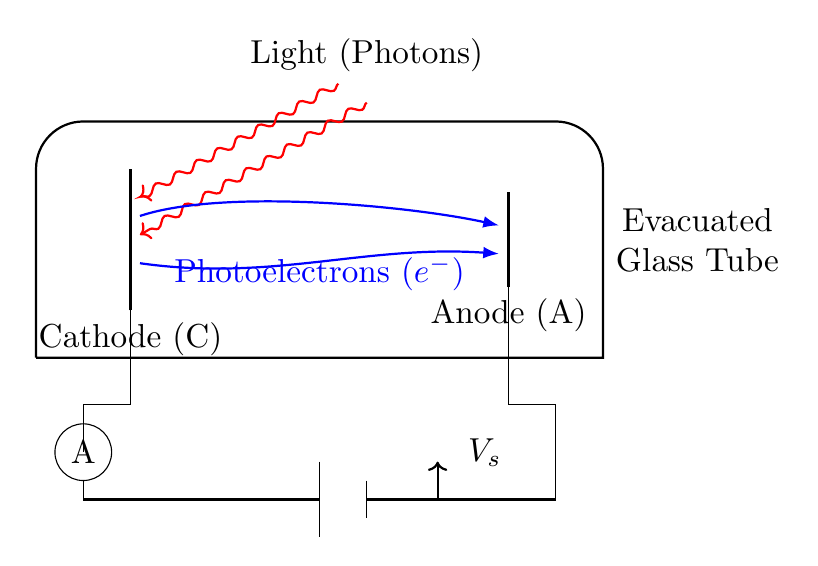
\begin{tikzpicture}[scale=1.2, transform shape]
        % Evacuated tube
        \draw[thick] (0,0) -- (0,2) arc (180:90:0.5) -- (5.5,2.5) arc (90:0:0.5) -- (6,0) -- (0,0);
        \node[align=center] at (7, 1.25) {Evacuated \\ Glass Tube};

        % Cathode (Emitter)
        \draw[fill=gray!30, thick] (1,0.5) -- (1,2);
        \node[below] at (1,0.5) {Cathode (C)};

        % Anode (Collector)
        \draw[fill=gray!30, thick] (5,0.75) -- (5,1.75);
        \node[below] at (5,0.75) {Anode (A)};

        % Incident Light (Photons) - MODIFIED
        \draw[->, thick, red, decorate, decoration={snake, amplitude=0.5mm, segment length=3mm}] (3.5, 2.7) -- (1.1, 1.3);
        \draw[->, thick, red, decorate, decoration={snake, amplitude=0.5mm, segment length=3mm}] (3.2, 2.9) -- (1.1, 1.7);
        \node[above] at (3.5, 2.9) {Light (Photons)};

        % Emitted Electrons
        \draw[->, blue, thick, -{Latex[length=2mm]}] (1.1,1.5) .. controls (2,1.8) and (4,1.6) .. (4.9,1.4);
        \draw[->, blue, thick, -{Latex[length=2mm]}] (1.1,1.0) .. controls (2.5,0.8) and (3.5,1.2) .. (4.9,1.1);
        % Photoelectron label - MODIFIED
        \node[below, blue] at (3, 1.2) {Photoelectrons ($e^-$)};

        % External Circuit
        \draw (1,-0.5) -- (1,0.5);
        \draw (5,-0.5) -- (5,0.75);
        \draw (1,-0.5) -- (0.5,-0.5);
        \draw (5,-0.5) -- (5.5,-0.5);
        
        % Ammeter
        \draw (0.5,-0.5) -- (0.5,-1);
        \draw (0.5,-1) circle (0.3);
        \node at (0.5,-1) {A};
        \draw (0.5,-1.3) -- (0.5,-1.5);
        
        % Variable Voltage Supply
        \draw (5.5,-0.5) -- (5.5,-1.5);
        \draw[thick] (5.5,-1.5) -- (3.5,-1.5);
        \draw (3.5, -1.3) -- (3.5, -1.7); % Short line of battery
        \draw (3, -1.1) -- (3, -1.9); % Long line of battery
        \draw[thick] (3,-1.5) -- (0.5,-1.5);
        \draw[thick, ->] (4.25,-1.5) -- (4.25, -1.1);
        \node at (4.75, -1.0) {$V_s$};

    \end{tikzpicture}
    \caption{Diagram of the photoelectric effect experiment.}
    \label{fig:photoelectric}
\end{figure}


\newpage
\section{Derivation of Radiation Pressure}
\label{sec:rad_pressure_derivation}

The concept of radiation pressure is built upon \textbf{Newton's Second Law}, which states that force is the rate of change of momentum, $F = \frac{\Delta p}{\Delta t}$. Pressure is then the force exerted over a specific area, $P_{\text{rad}} = \frac{F}{A}$.

\subsection{Case 1: Perfectly Absorbing Surface}
Imagine a beam of light shining perpendicularly onto a black surface that absorbs all incident photons.

\begin{enumerate}
    \item \textbf{Momentum of Photons:} A single photon with energy $E$ has a momentum $p_{\text{photon}} = E/c$.

    \item \textbf{Total Momentum Delivered:} The intensity ($I$) of the light beam is the energy delivered per unit area per unit time ($I = \frac{E}{A \cdot \Delta t}$). The total energy ($\Delta E$) hitting an area $A$ in a time interval $\Delta t$ is therefore $\Delta E = I \cdot A \cdot \Delta t$. The total momentum ($\Delta p$) carried by these photons and transferred to the surface upon absorption is:
    \[ \Delta p = \frac{\Delta E}{c} = \frac{I \cdot A \cdot \Delta t}{c} \]

    \item \textbf{Calculating the Force:} Using Newton's Second Law, the force on the surface is the total momentum transferred per unit of time:
    \[ F = \frac{\Delta p}{\Delta t} = \frac{\frac{I \cdot A \cdot \Delta t}{c}}{\Delta t} = \frac{I \cdot A}{c} \]

    \item \textbf{Calculating the Pressure:} Finally, we divide the force by the area $A$ to find the pressure:
    \[ P_{\text{rad}} = \frac{F}{A} = \frac{\frac{I \cdot A}{c}}{A} \]
    This simplifies to the final result for a perfectly absorbing surface:
    \begin{equation}
        P_{\text{rad}} = \frac{I}{c}
    \end{equation}
\end{enumerate}

\subsection{Case 2: Perfectly Reflecting Surface}
For a perfectly reflecting surface, the process is similar but with one crucial difference regarding the change in momentum.

When a photon hits the surface, it bounces back. If its initial momentum was $p$, its final momentum is $-p$ (in the opposite direction).

The \textbf{change} in the photon's momentum is:
\[ \Delta p_{\text{photon}} = p_{\text{final}} - p_{\text{initial}} = (-p) - (p) = -2p \]

By the law of conservation of momentum, if the photon's momentum changed by $-2p$, the momentum transferred \textit{to the surface} must be $\mathbf{+2p}$. This is double the momentum transfer compared to an absorbing surface.

Consequently, the reflecting surface experiences twice the force and twice the pressure:
\begin{equation}
    P_{\text{rad (reflecting)}} = \frac{2I}{c}
\end{equation}

\newpage
\section{Solved Problems (From SPhO Papers)}

\subsection{Question 1: SPhO 2022}
\begin{quote}
    In a photoelectric experiment, monochromatic ultraviolet light of wavelength \SI{60}{\nano\meter} and intensity \SI{0.7}{\watt\per\meter\squared} is incident onto a cathode which has a surface area of \SI{10}{\centi\meter\squared}. It is found that the photoelectric current decreases to zero when the anode has a negative potential of \SI{4.25}{\volt} with respect to the cathode. When the anode is at a positive potential with respect to the cathode, the saturation photoelectric current is \SI{21.7}{\nano\ampere}.
\end{quote}

\subsubsection*{(a) Calculate the linear momentum of the photoelectrons which are emitted with the maximum kinetic energy.}
\textbf{Solution:}
\begin{enumerate}
    \item \textbf{Find the maximum kinetic energy ($K_{\text{max}}$):}
    $K_{\text{max}} = eV_s = (\SI{1.602e-19}{\coulomb})(\SI{4.25}{\volt}) = \SI{6.8085e-19}{\joule}$.

    \item \textbf{Calculate the momentum ($p$):}
    $p = \sqrt{2m_e K_{\text{max}}} = \sqrt{2(\SI{9.11e-31}{\kilo\gram})(\SI{6.8085e-19}{\joule})} \approx \SI{1.114e-24}{\newton\second}$.
\end{enumerate}
\textbf{Final Answer:} The linear momentum is \textbf{\SI{1.114e-24}{\newton\second}}.

\subsubsection*{(b) What is the ratio of $\frac{N_{e}}{N_{p}}$?}
\textbf{Solution:}
\begin{enumerate}
    \item \textbf{Calculate the rate of incident photons ($N_p$):}
    $E_{\text{photon}} = \frac{hc}{\lambda} = \frac{(\SI{6.626e-34}{\joule\second})(\SI{3.00e8}{\meter\per\second})}{\SI{60e-9}{\meter}} = \SI{3.313e-18}{\joule}$.
    $P = I \cdot A = (\SI{0.7}{\watt\per\meter\squared})(\SI{10e-4}{\meter\squared}) = \SI{7.0e-4}{\watt}$.
    $N_p = \frac{P}{E_{\text{photon}}} = \frac{\SI{7.0e-4}{\joule\per\second}}{\SI{3.313e-18}{\joule}} \approx \SI{2.113e14}{\per\second}$.

    \item \textbf{Calculate the rate of emitted electrons ($N_e$):}
    $N_e = \frac{I_{\text{sat}}}{e} = \frac{\SI{21.7e-9}{\coulomb\per\second}}{\SI{1.602e-19}{\coulomb}} \approx \SI{1.355e11}{\per\second}$.
    
    \item \textbf{Find the ratio:}
    $\frac{N_e}{N_p} = \frac{\num{1.355e11}}{\num{2.113e14}} \approx \num{6.415e-4}$.
\end{enumerate}
\textbf{Final Answer:} The ratio is \textbf{\num{6.415e-4}}.

\subsubsection*{(c) What are the possible wavelengths of the photon emitted when the hydrogen atom de-excites?}
\textbf{Solution:}
\begin{enumerate}
    \item \textbf{Energy of the incident electron:} $K_{\text{max}} = \SI{4.25}{\electronvolt}$.
    \item \textbf{Minimum energy for excitation of Hydrogen:} The energy to excite from $n=1$ ($E_1 = \SI{-13.6}{\electronvolt}$) to $n=2$ ($E_2 = \SI{-3.4}{\electronvolt}$) is $\Delta E = E_2 - E_1 = \SI{10.2}{\electronvolt}$.
    \item \textbf{Compare energies:} The electron's energy (\SI{4.25}{\electronvolt}) is less than the required excitation energy (\SI{10.2}{\electronvolt}).
\end{enumerate}
\textbf{Final Answer:} The electron's energy is insufficient to excite the hydrogen atom. Therefore, \textbf{no emission is possible}.

\hrulefill
\subsection{Question 2: SPhO 2023}
\begin{quote}
A beam of monochromatic UV light with wavelength \SI{50}{\nano\meter} is incident onto a blackened flat plate of total area \SI{200}{\centi\meter\squared}. The beam has an intensity of \SI{24}{\watt\per\meter\squared}. Calculate the force exerted by the light beam.
\end{quote}
\textbf{Solution:}
\begin{enumerate}
    \item \textbf{Assumption:} The blackened plate is a perfect absorber.
    \item \textbf{Calculate radiation pressure ($P_{\text{rad}}$):} For absorption, $P_{\text{rad}} = \frac{I}{c} = \frac{\SI{24}{\watt\per\meter\squared}}{\SI{3.00e8}{\meter\per\second}} = \SI{8.0e-8}{\pascal}$.
    \item \textbf{Calculate the force ($F$):} $F = P_{\text{rad}} \cdot A = (\SI{8.0e-8}{\newton\per\meter\squared})(\SI{0.02}{\meter\squared}) = \SI{1.6e-9}{\newton}$.
\end{enumerate}
\textbf{Final Answer:} The force is \textbf{\SI{1.6e-9}{\newton}}.

\hrulefill
\subsection{Question 3: SPhO 2019}
\begin{quote}
A beam of monochromatic light of intensity \SI{50}{\watt\per\meter\squared} is incident normally onto a perfectly reflecting surface. Determine the pressure exerted.
\end{quote}
\textbf{Solution:}
\begin{enumerate}
    \item \textbf{Use the formula for a reflecting surface:} For perfect reflection, $P_{\text{rad}} = \frac{2I}{c}$.
    \item \textbf{Substitute values:} $P_{\text{rad}} = \frac{2(\SI{50}{\watt\per\meter\squared})}{\SI{3.00e8}{\meter\per\second}} \approx \SI{3.33e-7}{\pascal}$.
\end{enumerate}
\textbf{Final Answer:} The pressure is \textbf{\SI{3.33e-7}{\pascal}}.

\newpage
\section{New Practice Problems}

\subsection{Problem 1: The Photoelectric Effect on an Unknown Metal}
\begin{quote}
    Light with a wavelength of \SI{250}{\nano\meter} is incident on an unknown metal plate. The emitted photoelectrons are found to have a maximum kinetic energy of \SI{2.95}{\electronvolt}.
\end{quote}

\subsubsection*{(a) What is the work function of the metal in electron-volts (eV)?}
\textbf{Solution:}
\begin{enumerate}
    \item \textbf{Calculate photon energy ($E_{\text{photon}}$):} $E_{\text{photon}} = \frac{hc}{\lambda} = \frac{\SI{1240}{\electronvolt\nano\meter}}{\SI{250}{\nano\meter}} = \SI{4.96}{\electronvolt}$.
    \item \textbf{Calculate the work function ($\phi$):} $\phi = E_{\text{photon}} - K_{\text{max}} = \SI{4.96}{\electronvolt} - \SI{2.95}{\electronvolt} = \SI{2.01}{\electronvolt}$.
\end{enumerate}
\textbf{Final Answer:} The work function is \textbf{\SI{2.01}{\electronvolt}}.

\subsubsection*{(b) What is the cutoff wavelength ($\lambda_c$) for this metal?}
\textbf{Solution:}
\[ \lambda_c = \frac{hc}{\phi} = \frac{\SI{1240}{\electronvolt\nano\meter}}{\SI{2.01}{\electronvolt}} \approx \SI{617}{\nano\meter} \]
\textbf{Final Answer:} The cutoff wavelength is \textbf{\SI{617}{\nano\meter}}.

\hrulefill
\subsection{Problem 2: Solar Sail Propulsion}
\begin{quote}
    A small interplanetary probe has a mass of \SI{500}{\kilo\gram} and is propelled by a perfectly reflecting solar sail with an area of \SI{400}{\meter\squared}. The intensity of solar radiation is \SI{1360}{\watt\per\meter\squared}.
\end{quote}
\begin{figure}[h!]
    \centering
    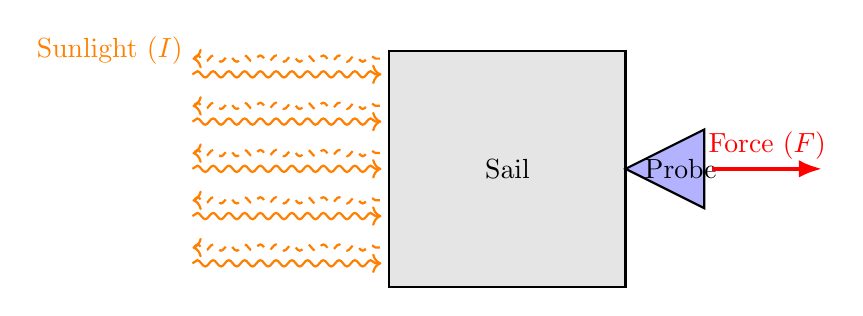
\begin{tikzpicture}[scale=1.0, transform shape]
        % Solar Sail
        \draw[fill=gray!20, thick] (-1.5, -1.5) rectangle (1.5, 1.5);
        \node at (0, 0) {Sail};

        % Probe Body
        \draw[fill=blue!30, thick] (1.5, 0) -- (2.5, 0.5) -- (2.5, -0.5) -- cycle;
        \node at (2.2, 0) {Probe};
        
        % Incident Photons (Sunlight)
        \foreach \y in {-1.2, -0.6, 0, 0.6, 1.2} {
            \draw[->, thick, orange, decorate, decoration={snake, amplitude=0.4mm, segment length=2mm}] (-4, \y) -- (-1.6, \y);
        }
        \node[left, orange] at (-4, 1.5) {Sunlight ($I$)};

        % Reflected Photons
        \foreach \y in {-1.2, -0.6, 0, 0.6, 1.2} {
            \draw[<-, thick, orange, dashed, decorate, decoration={snake, amplitude=0.4mm, segment length=2mm}] (-4, \y+0.2) -- (-1.6, \y+0.2);
        }
        
        % Force Vector
        \draw[->, -{Latex[length=3mm]}, ultra thick, red] (2.6, 0) -- (4, 0);
        \node[above, red] at (3.3, 0) {Force ($F$)};
    \end{tikzpicture}
    \caption{Diagram of a solar sail being propelled by radiation pressure.}
    \label{fig:solarsail}
\end{figure}
\subsubsection*{(a) What is the force exerted on the solar sail?}
\textbf{Solution:}
\begin{enumerate}
    \item \textbf{Calculate radiation pressure ($P_{\text{rad}}$):} $P_{\text{rad}} = \frac{2I}{c} = \frac{2(\SI{1360}{\watt\per\meter\squared})}{\SI{3.00e8}{\meter\per\second}} \approx \SI{9.07e-6}{\pascal}$.
    \item \textbf{Calculate the force ($F$):} $F = P_{\text{rad}} \cdot A = (\SI{9.07e-6}{\newton\per\meter\squared})(\SI{400}{\meter\squared}) \approx \SI{3.63e-3}{\newton}$.
\end{enumerate}
\textbf{Final Answer:} The force is \textbf{\SI{3.63e-3}{\newton}}.

\subsubsection*{(b) What is the initial acceleration of the probe?}
\textbf{Solution:}
\[ a = \frac{F}{m} = \frac{\SI{3.63e-3}{\newton}}{\SI{500}{\kilo\gram}} \approx \SI{7.26e-6}{\meter\per\second\squared} \]
\textbf{Final Answer:} The acceleration is \textbf{\SI{7.26e-6}{\meter\per\second\squared}}.

\hrulefill
\subsection{Problem 3: Excitation of Helium Ions}
\begin{quote}
    A stationary, singly-ionized helium atom ($He^+$) in its ground state ($n=1$) is struck by a photoelectron with kinetic energy of \SI{49.2}{\electronvolt}.
\end{quote}
\subsubsection*{(a) What is the highest energy level ($n$) that the $He^+$ ion can be excited to?}
\textbf{Solution:}
\begin{enumerate}
    \item \textbf{Calculate $He^+$ energy levels ($Z=2$) using $E_n = -Z^2 \frac{\SI{13.6}{\electronvolt}}{n^2}$:}
    \begin{itemize}
        \item $n=1: E_1 = -2^2 \frac{\SI{13.6}{\electronvolt}}{1^2} = \SI{-54.4}{\electronvolt}$
        \item $n=2: E_2 = -2^2 \frac{\SI{13.6}{\electronvolt}}{2^2} = \SI{-13.6}{\electronvolt}$
        \item $n=3: E_3 = -2^2 \frac{\SI{13.6}{\electronvolt}}{3^2} \approx \SI{-6.04}{\electronvolt}$
        \item $n=4: E_4 = -2^2 \frac{\SI{13.6}{\electronvolt}}{4^2} = \SI{-3.4}{\electronvolt}$
    \end{itemize}
    \item \textbf{Calculate excitation energies from ground state:}
    \begin{itemize}
        \item To $n=2: \Delta E_{1 \to 2} = E_2 - E_1 = \SI{40.8}{\electronvolt}$.
        \item To $n=3: \Delta E_{1 \to 3} = E_3 - E_1 = \SI{48.36}{\electronvolt}$.
        \item To $n=4: \Delta E_{1 \to 4} = E_4 - E_1 = \SI{51.0}{\electronvolt}$.
    \end{itemize}
    \item \textbf{Compare energies:} The electron's energy (\SI{49.2}{eV}) is greater than $\Delta E_{1 \to 3}$ but less than $\Delta E_{1 \to 4}$.
\end{enumerate}
\textbf{Final Answer:} The highest level is \textbf{$n=3$}.

\subsubsection*{(b) What are the possible wavelengths of photons emitted?}
\textbf{Solution:} The possible transitions are $3 \to 1$, $3 \to 2$, and $2 \to 1$.
\begin{figure}[h!]
    \centering
    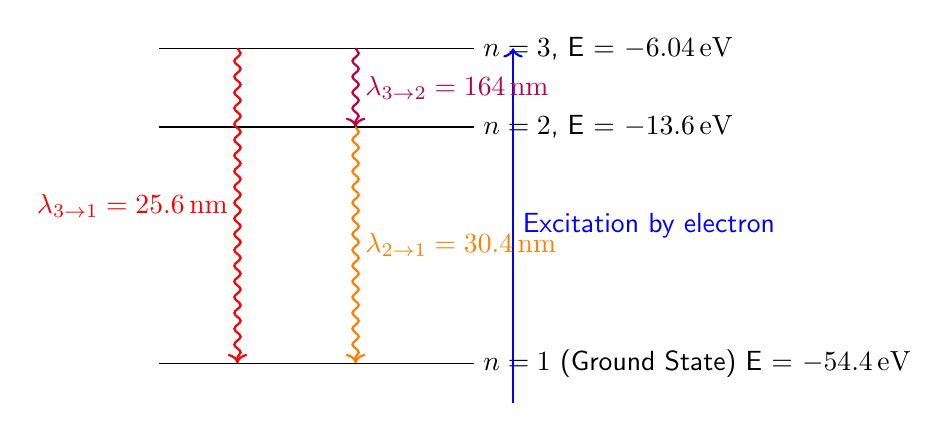
\begin{tikzpicture}[font=\sffamily]
        % Energy Levels
        \draw (0,0) -- (4,0) node[right] {$n=1$ (Ground State) E = \SI{-54.4}{\electronvolt}};
        \draw (0,3) -- (4,3) node[right] {$n=2$, E = \SI{-13.6}{\electronvolt}};
        \draw (0,4) -- (4,4) node[right] {$n=3$, E = \SI{-6.04}{\electronvolt}};
        
        % Excitation Arrow
        \draw[->, thick, blue] (4.5, -0.5) -- (4.5, 4);
        \node[right, blue] at (4.5, 1.75) {Excitation by electron};

        % De-excitation arrows and labels
        % 3 -> 1 transition
        \draw[->, thick, red, decorate, decoration={snake, amplitude=0.4mm, segment length=2mm}] (1,4) -- (1,0);
        \node[left, red] at (1,2) {$\lambda_{3 \to 1} = \SI{25.6}{\nano\meter}$};
        
        % 3 -> 2 transition
        \draw[->, thick, purple, decorate, decoration={snake, amplitude=0.4mm, segment length=2mm}] (2.5,4) -- (2.5,3);
        \node[right, purple] at (2.5, 3.5) {$\lambda_{3 \to 2} = \SI{164}{\nano\meter}$};
        
        % 2 -> 1 transition
        \draw[->, thick, orange, decorate, decoration={snake, amplitude=0.4mm, segment length=2mm}] (2.5,3) -- (2.5,0);
        \node[right, orange] at (2.5, 1.5) {$\lambda_{2 \to 1} = \SI{30.4}{\nano\meter}$};
        
    \end{tikzpicture}
    \caption{Energy level diagram for $He^+$ showing possible de-excitation pathways from the $n=3$ state.}
    \label{fig:he_levels}
\end{figure}
\begin{itemize}
    \item $\lambda_{3 \to 1} = \frac{hc}{\Delta E_{1 \to 3}} = \frac{\SI{1240}{\electronvolt\nano\meter}}{\SI{48.36}{\electronvolt}} \approx \SI{25.6}{\nano\meter}$.
    \item $\lambda_{3 \to 2} = \frac{hc}{E_3 - E_2} = \frac{\SI{1240}{\electronvolt\nano\meter}}{-6.04 - (-13.6)} \approx \SI{164}{\nano\meter}$.
    \item $\lambda_{2 \to 1} = \frac{hc}{\Delta E_{1 \to 2}} = \frac{\SI{1240}{\electronvolt\nano\meter}}{\SI{40.8}{\electronvolt}} \approx \SI{30.4}{\nano\meter}$.
\end{itemize}
\textbf{Final Answer:} The wavelengths are \textbf{\SI{25.6}{\nano\meter}}, \textbf{\SI{30.4}{\nano\meter}}, and \textbf{\SI{164}{\nano\meter}}.

\end{document}